% Source for the figure of EliasFano (sec. 22.6): the sequence 3, 4, 7,
% 13, 14, 15, 21, 43 in [0, 44), its low parts L of 3 bits and its high
% parts H in unary (1 for an item, 0 for the end of a bucket), and the
% access to x_6 (shaded). Build: make figures (in ../build).
\documentclass[border=4pt]{standalone}
\usepackage[T1]{fontenc}
\usepackage{lmodern}
\usepackage{amsmath}
\usepackage{tikz}
\usepackage{lamalunga}
% tikz-ads.tex: the TikZ styles shared by the figures of the memory of the
% manual, \input by each standalone figure: a cell of a vector (cell), the
% cell that an operation touches (touched), a free cell (free), a node of a
% linked structure (node), the labels of indices (index) and of variables
% (var), a pointer (ptr), and \cells and \indices to draw a row of cells.
\usetikzlibrary{arrows.meta,positioning,calc,fit,shapes.multipart}
\definecolor{adsTouched}{RGB}{214,196,236}
\definecolor{adsFree}{RGB}{236,236,236}
\tikzset{
  ads/.style={>={Stealth[length=2mm]},font=\small,
              every node/.append style={inner sep=0pt}},
  cell/.style={draw,minimum width=7mm,minimum height=7mm,
               font=\small\ttfamily,outer sep=0pt},
  touched/.style={cell,fill=adsTouched},
  free/.style={cell,fill=adsFree,text=black!45},
  node/.style={draw,rounded corners=1pt,minimum width=8mm,
               minimum height=6mm,font=\small\ttfamily},
  index/.style={font=\scriptsize\ttfamily,text=black!60},
  var/.style={font=\small\itshape},
  ptr/.style={->,thick}
}
% \cells{name}{x,y}{list}: a row of cells, the first at (x,y), named
% name-0, name-1, ...; each item is text/style, the style one of cell,
% touched and free (e.g., {a/cell,e/touched,/free})
\newcommand{\cells}[3]{%
  \foreach \v/\s [count=\i from 0] in {#3}
    \node[\s] (#1-\i) at ($(#2)+(\i*7mm,0)$) {\v};}
% \indices{name}{n}: the indices 0 .. n-1 under the cells of name
\newcommand{\indices}[2]{%
  \foreach \i in {0,...,\numexpr#2-1\relax}
    \node[index,below=1.2mm of #1-\i] {\i};}

\begin{document}

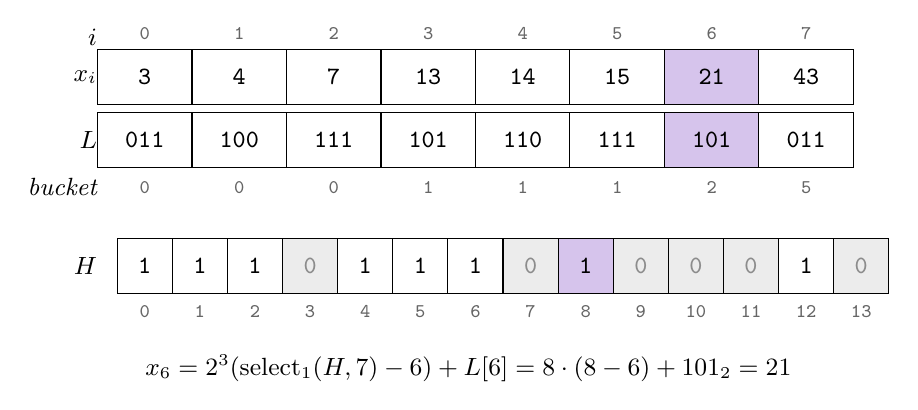
\begin{tikzpicture}[ads]
  \node[var,anchor=east] at (-6mm,0) {$x_i$};
  \node[var,anchor=east] at (-6mm,-8mm) {$L$};
  \node[cell,minimum width=12mm] (x0) at (0mm,0) {3};
  \node[cell,minimum width=12mm] (l0) at (0mm,-8mm) {011};
  \node[index,above=1.2mm of x0] {0};
  \node[cell,minimum width=12mm] (x1) at (12mm,0) {4};
  \node[cell,minimum width=12mm] (l1) at (12mm,-8mm) {100};
  \node[index,above=1.2mm of x1] {1};
  \node[cell,minimum width=12mm] (x2) at (24mm,0) {7};
  \node[cell,minimum width=12mm] (l2) at (24mm,-8mm) {111};
  \node[index,above=1.2mm of x2] {2};
  \node[cell,minimum width=12mm] (x3) at (36mm,0) {13};
  \node[cell,minimum width=12mm] (l3) at (36mm,-8mm) {101};
  \node[index,above=1.2mm of x3] {3};
  \node[cell,minimum width=12mm] (x4) at (48mm,0) {14};
  \node[cell,minimum width=12mm] (l4) at (48mm,-8mm) {110};
  \node[index,above=1.2mm of x4] {4};
  \node[cell,minimum width=12mm] (x5) at (60mm,0) {15};
  \node[cell,minimum width=12mm] (l5) at (60mm,-8mm) {111};
  \node[index,above=1.2mm of x5] {5};
  \node[touched,minimum width=12mm] (x6) at (72mm,0) {21};
  \node[touched,minimum width=12mm] (l6) at (72mm,-8mm) {101};
  \node[index,above=1.2mm of x6] {6};
  \node[cell,minimum width=12mm] (x7) at (84mm,0) {43};
  \node[cell,minimum width=12mm] (l7) at (84mm,-8mm) {011};
  \node[index,above=1.2mm of x7] {7};
  \node[var,anchor=east] at (-6mm,5mm) {$i$};
  \node[var,anchor=east] at (-6mm,-14mm) {bucket};
  \foreach \b [count=\i from 0] in {0,0,0,1,1,1,2,5}
    \node[index] at (\i*12mm,-14mm) {\b};
  \node[var,anchor=east] at (-6mm,-24mm) {$H$};
  \node[cell] (h-0) at (0mm,-24mm) {1};
  \node[cell] (h-1) at (7mm,-24mm) {1};
  \node[cell] (h-2) at (14mm,-24mm) {1};
  \node[free] (h-3) at (21mm,-24mm) {0};
  \node[cell] (h-4) at (28mm,-24mm) {1};
  \node[cell] (h-5) at (35mm,-24mm) {1};
  \node[cell] (h-6) at (42mm,-24mm) {1};
  \node[free] (h-7) at (49mm,-24mm) {0};
  \node[touched] (h-8) at (56mm,-24mm) {1};
  \node[free] (h-9) at (63mm,-24mm) {0};
  \node[free] (h-10) at (70mm,-24mm) {0};
  \node[free] (h-11) at (77mm,-24mm) {0};
  \node[cell] (h-12) at (84mm,-24mm) {1};
  \node[free] (h-13) at (91mm,-24mm) {0};
  \foreach \i in {0,...,13}
    \node[index,below=1.4mm of h-\i] {\i};
  \node[var,anchor=west] at (0,-37mm)
    {$x_6 = 2^3 ( \mathrm{select}_1( H , 7 ) - 6 ) + L[ 6 ] = 8 \cdot ( 8 - 6 ) + 101_2 = 21$};
\end{tikzpicture}
\end{document}
